%! Date = 28/03/2023

% Preamble
\documentclass[a4paper,12pt]{article}

\usepackage[utf8]{inputenc}
\usepackage[T1]{fontenc}
\usepackage{lmodern}
\usepackage[english]{babel}
\usepackage{graphicx}
\usepackage[style=authoryear]{biblatex}
\usepackage{url}
\usepackage{hyperref}
\usepackage{booktabs}
\usepackage{tabularx}
\addbibresource{references.bib}

\begin{document}
    \begin{titlepage}
        \begin{center}
        {\huge\bfseries Suitability of an Internal Developer Portal to Support the Daily Work of BizDevOps Engineers\par}
            \vspace{2cm}

            {\scshape\large Certificate work in the \par}
            {\scshape\large CAS Digital Product Lead \par}
            \vspace{1cm}

            {\scshape\large HWZ University of Applied Sciences \par}
            {\scshape\large for Business Administration Zurich \par}
            \vspace{4cm}

            {\normalsize submitted to\par}
            \vspace{0.5cm}

            {\large Ralph Hutter\par}
            \vfill
            {\normalsize submitted by\par}
            \vspace{0.5cm}
            {\large Thierry Peng\par}
            \vspace{0.5cm}
            {\normalsize Address: placeholder 68, placeholder\par}
            {\normalsize  Place, Date: placeholder, \today\par}

        \end{center}
    \end{titlepage}


    \section*{Management Summary}
    %TODO
    \pagebreak


    \tableofcontents
    \pagebreak

    \section*{Used Tools}
    In addition to the sources mentioned in the bibliography\ref{sec:bibliograhpy}, the following aids and tools have been used
    \begin{itemize}
        \item Version control with Git and GitHub, the source code for this document is at \url{https://github.com/thpeng/mas/tree/master/src/mca-dpl23-1}
        \item Deepl at (\url{https://www.deepl.com/}) for supporting translations.
        \item Microsoft Forms for conducting a survey (\url{https://forms.office.com}) .
        \item The document has been written with \LaTeX  (\url{https://miktex.org/}) and using IntelliJ IDEA (\url{https://www.jetbrains.com/de-de/idea/})
    \end{itemize}

    \section*{Declaration of Honour}

    I hereby confirm that I have
    \begin{itemize}
        \item prepared the present thesis independently and without the use of sources or aids other than those indicated,
        \item identified the sources used as such, either verbatim or in terms of content,
        \item not yet submitted this work in the same or similar form to an examination board.
    \end{itemize}
    Bern, \today\newline
    \newline
    \newline
    \newline
    \begin{tabular}{@{}p{5.0cm}@{}}
        \hrulefill \\
        Thierry Peng
    \end{tabular}

    \pagebreak

    % max 15 - 20 pages beginning here


    \section{Introduction}
    \label{sec:introduction}
    SBB has an extensive and constantly growing IT landscape of applications and tools for supporting the digitization
    of core business processes of the SBB .
    This digitization efforts brought great changes into the IT department of the SBB.
    In less than ten years, the development model has changed from strictly waterfall to an agile methodology, cloud
    technologies have been adopted while hardware-bound platforms are being out-phased and a new internal organization,
    on the base of separation of specialist and line management, has been introduced.
    While these changes are taking root now and are yielding various positives results, they still pose a challenge
    because of new as well as still-existing complexity and the rapidly changing technological landscape.
    In addition, regulatory pressure has increased significantly in recent years, as exemplified by the
    HCBöV\footnote{Handbuch Cybersecurity für Betriebe des öffentlichen Vekehrs}, as well as the new Data Protection Act
    in Switzerland - nDSG.\linebreak
    Feedback from various employees in different roles from SBB's so called ``Digitalen Zone`` indicates, that the overall
    increase in complexity has an impact on the daily work of DevOps\footnote{DevOps is a combination of the words
    Development and Operations and can be either a role or a set of practices} engineers.
    The picture that is being painted is, although all information for the design, development and operation of
    applications is available in principle, it is maintained in very different places and forms.
    This makes the procurement of information for these activities time-consuming and requires that a DevOps
    engineer is already very familiar with the IT landscape of SBB .

    \subsection{Problem Statement and Controversy}
    \label{subsec:iproblemstatement}
    Research on the Internet about the problem, as well as advice from suppliers, shows that there is greater momentum
    to address such issues with an Internal Developer Portal (IDP). The central promise of the concept of an
    Internal Developer Portal is that it can reduce the so-called ``cognitive load`` of DevOps engineers by easily
    processing and presenting information about teams, associated applications and their use of infrastructure.

    \subsection{Objective of the Certificate Work}
    \label{subsec:iobjective}
    The purpose of this certificate thesis is to examine whether the above-mentioned problem is valid and if true,
    can be addressed and to what extent by introducing an Internal Developer Portal.
    The first step is to discover the value proposition by the concept of an Internal Developer Platform and putting this
    proposition in the general context of developing software and operating IT systems.
    The second step is to corroborate the problem statement about complexity and lacking integration with a quantitative
    survey.
    The third part will be to put the results of the survey and the value proposition together and to recommend a course
    of action.


    \section{Value Proposition for an Internal Developer Portal}
    \label{sec:vp}
    An Internal Developer Portal is a web-based information catalogue which is tailored for the needs of
    engineers operating IT systems, developing software and other related work.
    Internal Developer Portal are proposed as the solution for perceived problems\parencite{backstagestory} of DevOps
    engineers while developing and operating IT Systems such as
    \begin{itemize}
        \item A lack of a central repository for reliable and tailored information
        \item A high cognitive load of engineers because of switching between multiple and very different tools while developing or operating IT Systems
        \item Increasing the developer experience by abstracting away complexity in infrastructure management
    \end{itemize}
    One potential source of information for using in the Internal Developer Portal is an Internal Developer Platform.

    \subsection{Internal Developer Platform}
    \label{subsec:vpplatform}
    Gartner makes a differentiation between the concept of an Internal Developer Portal and an Internal Developer Platform:
    ``internal developer portals serve as the interface through which developers can discover and
    access internal developer platform capabilities``\parencite{gartner} .
    An Internal Developer Platform (Platform), according to the COO Christoph C. Richter from Humanitec\parencite{richteretal} ,
    should consist at least of the following component:
    \begin{itemize}
        \item Application Configuration Management
        \item Infrastructure Orchestration
        \item Environment Management
        \item Deployment Management
        \item Role-Based Access Control
    \end{itemize}
    In some other sources, there are also additional components mentioned, e.g. Observability\parencite{xenon}.
    XENONSTACK as well as Humanitec mentioned before, are suppliers of Internal Developer Platform solutions with
    different capabilities.
    The capabilities and components of Internal Developer Platforms are not unique to the products of those two suppliers.
    In most contemporary IT operations or software development departments these components and practices are well-known
    and used widely.
    Beyond the size of a very small team, it is necessary to use tooling to know where, in which version and with what
    configuration a software artifact was installed.
    The reason behind this may be to coordinate a new software rollout, test the software on a dedicated stage, fix bugs
    or develop new features and to solve incidents caused by your software.
    Thus, it can be argued, that the concept of an Internal Developer Platform is not unique to specific products
    or offerings, but can be used on a set of tooling and practices supporting IT operations and software development.
    This set of tooling and practices can be viewed as predecessors of Internal Developer Platforms and are usually
    distinct solutions or products.
    For example there is a separate Configuration Management Database
    to address the need of Application Configuration Management or there is a purpose built Continuous Integration /
    Continuous Deployment pipeline for addressing the need for a Deployment Management.
    These solutions are not necessarily integrated with each other.
    It may be also the case, that these
    products or solutions were established before the advent of Agile Methodologies and DevOps.

    \subsection{DevOps}
    \label{subsec:devops}
    With DevOps, the classical disciplines of IT operating and software development are much more integrated to reduce
    friction, release features more often and to improve quality of the products\parencite{safedevops}.
    Before DevOps, it was quite common to have different tooling for either development or operating roles, usually
    because those two roles were separated in different departments or teams.
    One of the fundamental principle of DevOps was coined by the current CTO of Amazon, Werner Vogels;
    ``you build it, you run it``\parencite{vogels} .
    This means, that the same team that develops the software, operates it.
    With DevOps, a team takes the full responsibility over the lifecycle for a software or a platform.
    In combination with agile methodologies such as Scrum\footnote{Scrum is a iterative software development methodology}
    or SAFe\footnote{SAFe stands for Scaled Agile Framework and adds orchestration layers above agile (Scrum) teams for
    a better cross-team and product-centric alignment} even business oriented people are integrated in this
    cross-functional team.
    One example of a business oriented role in a DevOps team is the Product Owner\parencite{safepo} .
    This has also the implication, that a team must have a wide range of skills and should have access to different
    tools needed for their work.
    Such tools can be needed for activities such as requirements engineering, solution architecting, software development
    but also everything that is necessary to operate the software.
    Especially the operating of the software is a tool-intensive work.
    There are tools for logging, monitoring, incident handling and alarming.
    In the case of an incident, a configuration management database or an enterprise architecture database are crucial
    to find out to whom belongs a particular application or resource.
    This information is crucial to pinpoint a root cause and to resolve the incident quickly.
    While DevOps has various benefits, it adds quite a complexity for a team member in an agile and DevOps team.
    That's where the Integrated Developer Portal has various proposals to support the individual and the team in their
    daily business.

    \subsection{Internal Developer Portal}
    \label{subsec:vpportal}
    Manjunath Bhat from Gartner argues, that an Internal Developer Portal has three main characteristics\parencite{gartner}:
    \begin{itemize}
        \item Abstraction
        \item Developer-centric view
        \item Pluggable framework
    \end{itemize}
    The overarching goal of these characteristics are to increase the devops experience by shortening the time searching
    and interpreting information.
    The search task is supported by a central software catalogue.
    The interpretation of the data is supported by an underlying logical model, which describes the assets, technologies
    and their relationship in between.
    The logical model is different between each of the internal developer portal but have some common elements.

    \subsubsection{Vendors and Products}
    \label{sssec:vendors}
    While it's not the focus of this certificate work to delve into the details of each possible product on the market
    and make a comparison between them, it's worthwhile to describe a few.
    Redpoints mentions five products as ``Universal Service Catalogue`` offerings\parencite{devportalsprimer}.
    This kind of Internal Developer Portal is not tied into specific cloud offerings such as AWS, Azure or Google
    Cloud Platform (``API Catalog tied to an API Gateway / Service Mesh``)and has no opinion about a particular application
    architectural style, such as the products mentioned in the category ``Microservice Catalog``.
    \begin{table}[!htbp]
        \begin{center}
            \begin{tabularx}{\textwidth}{lllll}
                \toprule
                Vendor   & Product      & Year & License               & Deployment  \\
                \midrule
                Spotify  & backstage.io & 2020 & open source           & self-hosted \\
                Lyft     & clutch.sh    & 2020 & open source           & self-hosted \\
                Moment   & moment.dev   & Beta & proprietary           & SaaS        \\
                Opslevel & opslevel.com & 2018 & partially open source & SaaS        \\
                \bottomrule
            \end{tabularx}
        \end{center}
    \end{table}
    Roadie is omitted from the table because it's a commercial offering of Backstage.
    It seems, there are two main directions; Backstage and Clutch have been developed by two big tech companies for their
    internal audience, have been made available as opensource and Moment
    and OpsLevel are purposefully built by startups as a product and have commercial offerings.
    For the further discussion about the value proposition of an Internal Developer Portal, some screenshots and concepts will
    be used from Backstage.
    Backstage has been built by Spotify, which invests heavily in what they call the
    ``developer experience`` (DX)\parencite{spotifydx}.
    Additionally, Backstage was adopted in 2020 as an incubating project into the Cloud Native Computing Foundation\parencite{cncf} .

    \subsubsection{Discoverability}
    The Software Catalogue is the main feature of an Internal Developer Portal.
    Its purpose is to make the capabilities of the Internal Developer Platform accessible for an engineer as seen in the
    screenshot at\ref{fig:catalog}.

    \begin{figure}
        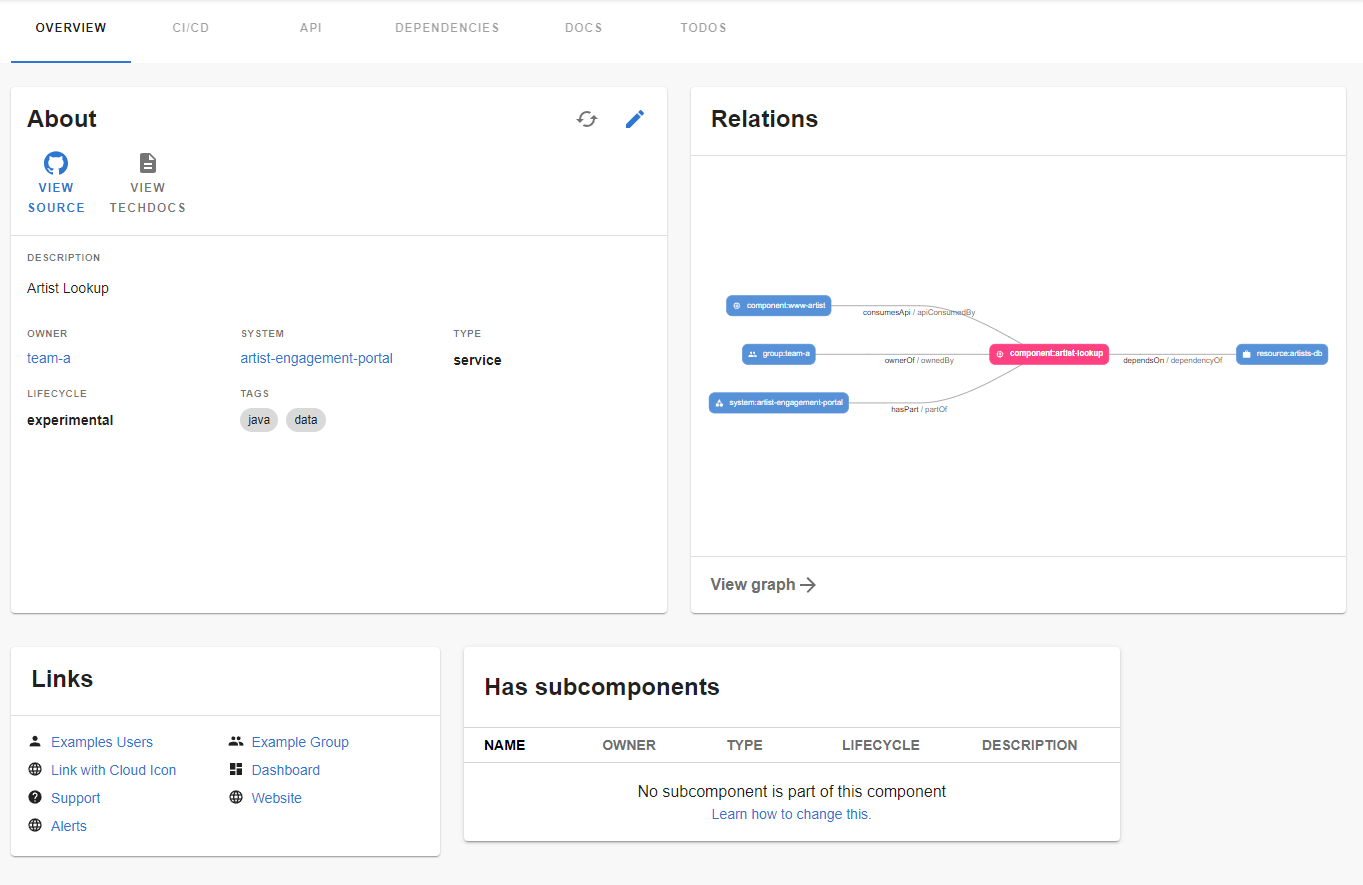
\includegraphics[width=\linewidth]{backstage_item_details}
        \caption{The Software Catalog from the Backstage Demo\parencite{backstagedemo}}
        \label{fig:catalog}
    \end{figure}
    Its content may be any combination of
    \begin{itemize}
        \item Teams with members
        \item Applications
        \item Infrastructure and platforms
        \item Most importantly, the relationships between those. These attributes are modelled, e.g. an application is owned by a team.
    \end{itemize}
    Data may be shown in a tabular fashion or may be shown as a relationship graph and the catalogue is searchable.
    An Engineer may bookmark its favourite items and its own resources are marked by ``owned``.

    In addition to the catalogue with its tabular overview, there is a details view.
    \begin{figure}
        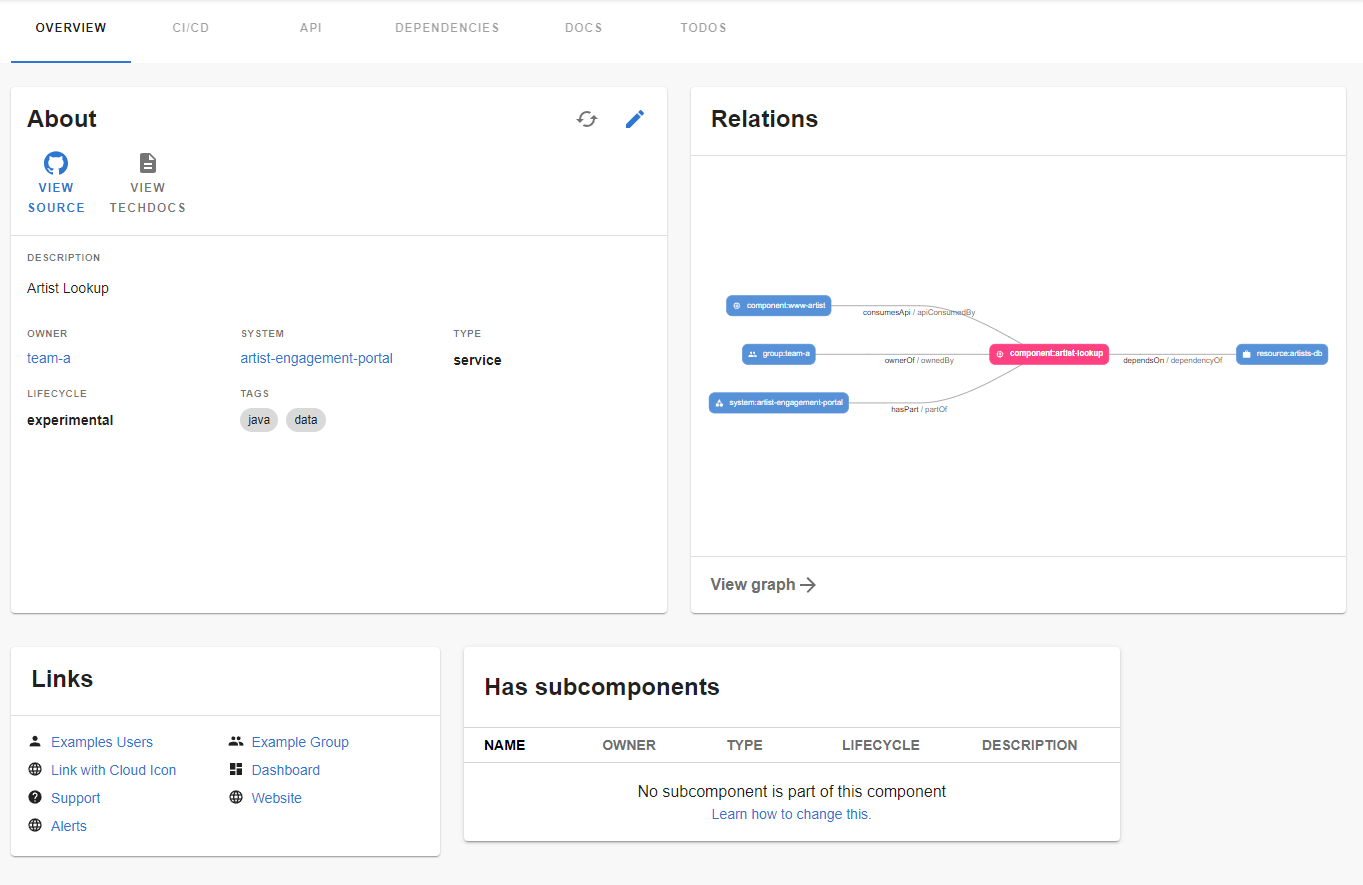
\includegraphics[width=\linewidth]{backstage_item_details}
        \caption{Details about an artifact}
        \label{fig:portaldetails}
    \end{figure}
    In the details view more attributes are shown for the chosen item from the overview.
    Depending on the kind of item, different attributes are shown.
    For an application, it may be its used resources, consumed and provided APIs and other subcomponents.
    For teams, the members are shown and its owned resources and its contact details.

    \subsubsection{Platform as a Product}
    In some implementations of an Internal Developer Portal, the catalogue is not merely a copy of an architecture database.
    In addition to the mentioned applications, platforms, organisational data and resources, there are other products
    of the teams shown.
    For example platform teams may offer support and consultation for their platform or area of expertise and advertise
    this service there.
    Some teams use the Internal Developer Platform to showcase code or libraries and thus create an inner-source community.
    In some cases, the whole lifecycle of a resource, from ordering, updating until removal are implemented or integrated
    in an Internal Developer Platform.
    In a know-how sharing session between SBB and Booking.com, Booking.com told about their Internal Developer Portal as a
    distinct product, which is owned by a dedicated team.
    This team is also responsible for the onboarding of other platform and application teams and entices them with the
    value of an integrated Internal Developer Portal.

    \subsubsection{Golden Path}
    The term ``Golden Path`` was coined by Spotify\parencite{spotifygoldenpath} and is itself a reference to the Frank
    Herberts Dune trilogy, describing the only viable path to getting things right.
    A Golden Path is a ready-to-use template for getting a project quickly started.
    It may consist of software engineering artifacts, pre-configured infrastructure components and is usually highly
    opinionated.
    Opinionated means, that the context of the company is already factored in, such as internal regulations,
    the currently promoted tech stack and other internal specifics.
    For example, a Golden Path for a database is already integrated with the security infrastructure of the company,
    logging is taken care of and some best practices concerning database configuration and modelling are implemented.
    Golden Pathes are not necessarily product-specific, they may encompass a typical development stack used
    in the company, such as a web application Golden Path consisting of a frontend build with javascript, a Java backend
    and an Oracle database, all integrated in a single build pipeline for CI/CD\footnote{CI/CD stands for continuous
    integration and continuous deployment and is a practice in software engineering. Its main focus is to automate all steps
    between development and rolling out on production, such as testing, building artifacts and installing them. Its goal
    is to deliver fast and with a high quality software to the client.}, securely configured and with the
    company look and feel already set up.
    With such a template mechanism in place, new applications ar built faster, reuse the same solutions for cross-cutting
    functionalities and relieve developers from writing tedious plumbing code to integrate each of these components with
    each other.

    \subsubsection{Technical Documentation}
    Platforms using an Internal Developer Portal may choose to migrate their user facing documentation to the Internal
    Developer Portal.
    The foundation for this technical documentation may be a solution based on markdown\parencite{backstagetechdocs}
    or similar syntax.
    The benefit with this approach is, that documentation is treated as code and can be integrated in the same toolchain.
    For example the documentation resides beside the code, can be peer-reviewed, built and released in the same manner.

    \subsubsection{Expertise}
    Splunk\footnote{Splunk is a company specialised in creating software for loganalysis and monitoring and it is known
    for its product with the same name}
    describes a use case, how to leverage an Internal Developer Platform to make expertise visible in their
    company\parencite{splunkidp} .
    Their solution is to enrich teams and users with additional data about their knowledge and let other user give feedback
    how a team or user did support them, called a ``Bravo`` in their terminology.
    Thus, they create something like a social network inside their company for connecting people to solve problems or
    easing the way how to find people with specific skills or knowledge.

    \subsubsection{Extendability}
    As shown in chapter\ref{sssec:vendors} , there are multiple offerings of Internal Developer Portal and varying
    implementations.
    In case of the Software-as-a-service offerings, the extendability consists of using plugins for well-known
    technologies or products and preparing and inserting the companies data for the catalogue feature.
    The self-hosted variants, such as Backstage and Clutch are more like a skeleton or a framework.
    For both products, there are pre-built binaries which are installable and runnable, but you can choose to build your
    own Internal Developer Portal and use these products as a starting point.
    Both support custom-made plugins on the front-end side which may use additional datasource outside the direct
    internal developer portal.
    This approach is handy for decentralized organisational forms where each team have maximal autonomy about how they
    reach their goals, but would like to use and contribute to a centralized catalogue by adding data and functionality
    via plugins.
    The plugin architecture allows to leverage your Internal Developer Portal with the tooling landscape in a
    single and integrated user experience for DevOps Engineers.

    \subsubsection{FinOps}
    %TODO
    \pagebreak


    \section{Situation at the SBB IT}
    \label{sec:sbbit}
    The IT department of the Swiss Federal Railways (SBB) consists of around 1300 specialists and is responsible for
    700 applications\parencite{sbbitkennzahlen}.
    The applications built and operated by this department are used for a wide range of use cases.
    For example, some applications are covering generic enterprise use cases such as human resource management, finance
    and controlling.
    Other software is specially built for mission-critical, day-to-day operations of the railway such as the Rail Control
    System (RCS)\parencite{sbbrcs} .
    An SBB IT application may be a purchased product, may be developed in-house or is a combination thereof which is
    sometimes called a ``customization``.
    Applications and products, built and operated by the SBB, are regulated by different standards and regulations of the
    swiss government or by industry initiatives.
    Examples are the EN 50128 standard by the European Committee for Electrotechnical Standardization (CENELEC)\parencite{cenelec},
    which governs among other things the development of safety-related software with different requirement levels
    or the HCBöV\parencite{hcboev} with regulations concerning cyber-security, risk management, business continuity
    management among others.
    In addition to the more business-oriented applications, there is a need for platforms and tools to help create
    and operate these.
    Examples are a PaaS\footnote{A platform-as-a-service (PaaS) is a platform which exposes resources such as compute or
    storage to applications. The team which is building an application is relieved from the burden of obtaining and
    provisioning resources on a hardware level. A well-known implementation of a PaaS is Kubernetes from the CNCF.},
    databases, messaging but also networking, monitoring, security and
    speciality services like UX or test-engineering and others.

    \subsection{Internal Developer Platform}
    \label{subsec:sbbplatform}
    The SBB IT has for most of the core components of an Internal Developer Platform, as laid out in chapter\ref{subsec:vpplatform},
    already solutions in place:
    \begin{itemize}
        \item Application Configuration Management - is centered around the practice of GitOps\parencite{hashicorpvault}
        \item Infrastructure Orchestration - for example, SBB uses OpenShift since 2015\parencite{rhsbbopenshift}
        \item Environment Management - provided by OpenShift and CI/CD Pipelines
        \item Deployment Management - is provided by CI/CD pipelines built on Tekton and ArgoCD\parencite{sbbtekton}
        \item Role-Based Access Control - built-in in most of the SBB IT platforms
    \end{itemize}
    In addition, there are several other tools and applications used for the day-to-day operations and development.
    Most notable are the following
    \begin{itemize}
        \item Development and operation are dependent on a Wiki Software for documentation and communication.
        \item An Enterprise Architecture Database contains the information about used technologies, platforms and
        dependencies, as modelled by the architects
        \item An IT Service Management Platform contains the data concerning team contact information and support groups for applications
        \item A Configuration Management Database contains data about used assets, resources and relations to applications
    \end{itemize}
    Thus, it could be argued, that the foundation for an Internal Developer Platform is in place, but there are two
    critical pieces missing.
    First, most of the components mentioned are only partially integrated with each other.
    Examples for missing integration are different identifier for assets, unaligned authorization such as per-user vs.
    per-group models and manual data maintenance.
    Second, there is no central view to aggregate data contained in these applications and tools for the benefit of
    the DevOps engineers.

    \subsection{DevOps}
    \label{subsec:sbbdevops}
    In 2015 the practice of DevOps and a PaaS was first introduced in the SBB IT .
    The stated goals of these additions was to solve the rising complexity in operations and the perceived low velocity
    in responding to change\parencite{sbbdevops} .
    Four years later, a reorganisation brought a new operating model to the SBB IT, based on agile principles, DevOps and SAFe
    and created the role of the BizDevOps engineer\parencite{sbbagile} .
    Most pre-reorganisation roles such as an application engineer, operations manager, test engineer or a requirements engineer
    were converted to this BizDevOps Engineer role.
    Even some former business oriented roles are now called BizDevOps engineers and are integrated in this cross-functional
    teams.
    DevOps teams in 2023 are now the established standard, but they are still working mostly with tools for developing and
    operating from the organization before.
    While the tools itself may be the state of the art in their fields, they weren't bought or built with an end-to-end
    integration in mind which would benefit a BizDevOps engineer.

    \subsection{Internal Developer Portal}
    \label{subsec:sbbportal}
    Most BizDevOps teams of the SBB help themselves with some kind of organization for the necessary information
    for the day-to-day work.
    A common approach is to leverage the internal Wiki software, where each teams maintain their relevant http link
    collection in the context of their project in one or more pages.
    When someone joins a team, its first task is in most cases, that he/she must familiarize himself/herself with this
    collection.
    Naturally, these link collection grow outdated and its maintenance needs also effort from a team.
    If whole teams are being staffed, for example with models such as managed capacity or near-shore, it is even worse
    for getting up to speed.
    While this problem about discovery and sharing knowledge isn't fully addressed, there were some efforts to create
    a self-service portal for ordering resources.
    The reason for this portal was, that platform teams weren't happy with unstructured ordering with email, telephone or
    others ad-hoc methods and built a modular and decentralized portal for this use case.
    However, there was no single owner of the portal and after the immediate pain point of the platform has been adressed,
    there was no further effort to expand the functionality until now.


    \section{Method}
    \label{sec:method}
    The method chosen to verify the observations about the state of the DevOps Experience and to evaluate the value proposition
    of an Internal Developer Portal, is to hold a survey.
    The survey is created with a customer journey based on different BizDevOps personas.
    The personas and the customer journey are based on a preliminary, internal work\parencite{sbbjobstobedone}.

    \subsection{Customer Journey}
    \label{subsec:cusjour}
    The customer journey is focused on the interaction of different personas with the existing Internal Developer Platform.
    The assumption is, that this interaction between the BizDevOps Engineers and the Internal Developer Platform has a big
    impact on the DevOps Experience.
    The personas of the customer journey are roles which are quite common in a BizDevOps team in the SBB IT.\\
    \textit{Peter Plattform} is working as a platform engineer and interested in the lifecycle of resources and platforms which
    are necessary for the building and operating of application in his team.\\
    \textit{Diego Developer} is a software engineer and his duty is to work on features and enables in the context of his team.
    He is interested in building solutions and need knowhow and consulting for doing so.
    His secondary interest is, to get his work as fast as possible and with the highest quality into the production environment.
    \textit{Norbert Neuling} is the rookie in the team.\\
    He wants to acquire knowledge, try out the established technologies or platforms and needs a solid template for creating
    his own solutions.\\
    \textit{Agnes Architekt} is working as an IT architect.
    The product owner of the team asked her to identify variants to lower the operation cost.
    She is also very interested
    to know about changes in the platforms, so that she can inform the product owner and put the necessary enablers in
    the next product increment\footnote{SAFe terminology for a cycle of usually five two-week SCRUM Sprints of agile software development.}.\\
    \textit{Ida Incident} is working on an operational issue.
    She needs to know the technical topology of her application and the used platforms.
    She has to know, which team is responsible for which platform and how she could reach them.\\
    For more information, see figure\ref{fig:customerjourney}

    \subsection{Quantitative Survey}
    The goal of the survey is to
    %TODO Umfrage.

    \subsubsection{Question}
    For the survey 19 questions were created.
    17 are rating questions with a one star to five star range.
    One question was a question with a free text answer to solicit more input and to generate additional interview partner
    for a qualitative survey.
    These interviews and the resulting insights are not part of this certificate work.
    The final question was about the
    %TODO Umfrage.

    \subsubsection{Setup}
    The survey is made with Microsoft Forms.
    The audience of the survey are the subscribers of the main blog of the SBB IT platforms, CLEW\footnote{CLEW stands for Cloud, ESTA, itself an acronym of Entwicklungstack and WZU, Werkzeugunterstützung}.
    There are 784 subscriber on the blog.
    The start date of the survey was the 24.04.2023 and the end date was on 08.05.2024.

    \subsubsection{Result}
    %TODO Umfrage.


    \section{Conclusion}
    \label{sec:conclusion}
    \pagebreak
    % max 15 - 20 pages end here


    \section{List of Sources}
    \label{sec:bibliograhpy}
    \printbibliography[heading=none]


    \section{Appendix}
    \label{sec:appendix}

    \subsection{Customer Journey Map}
    \label{subsec:cusjourmap}
    \begin{figure}
        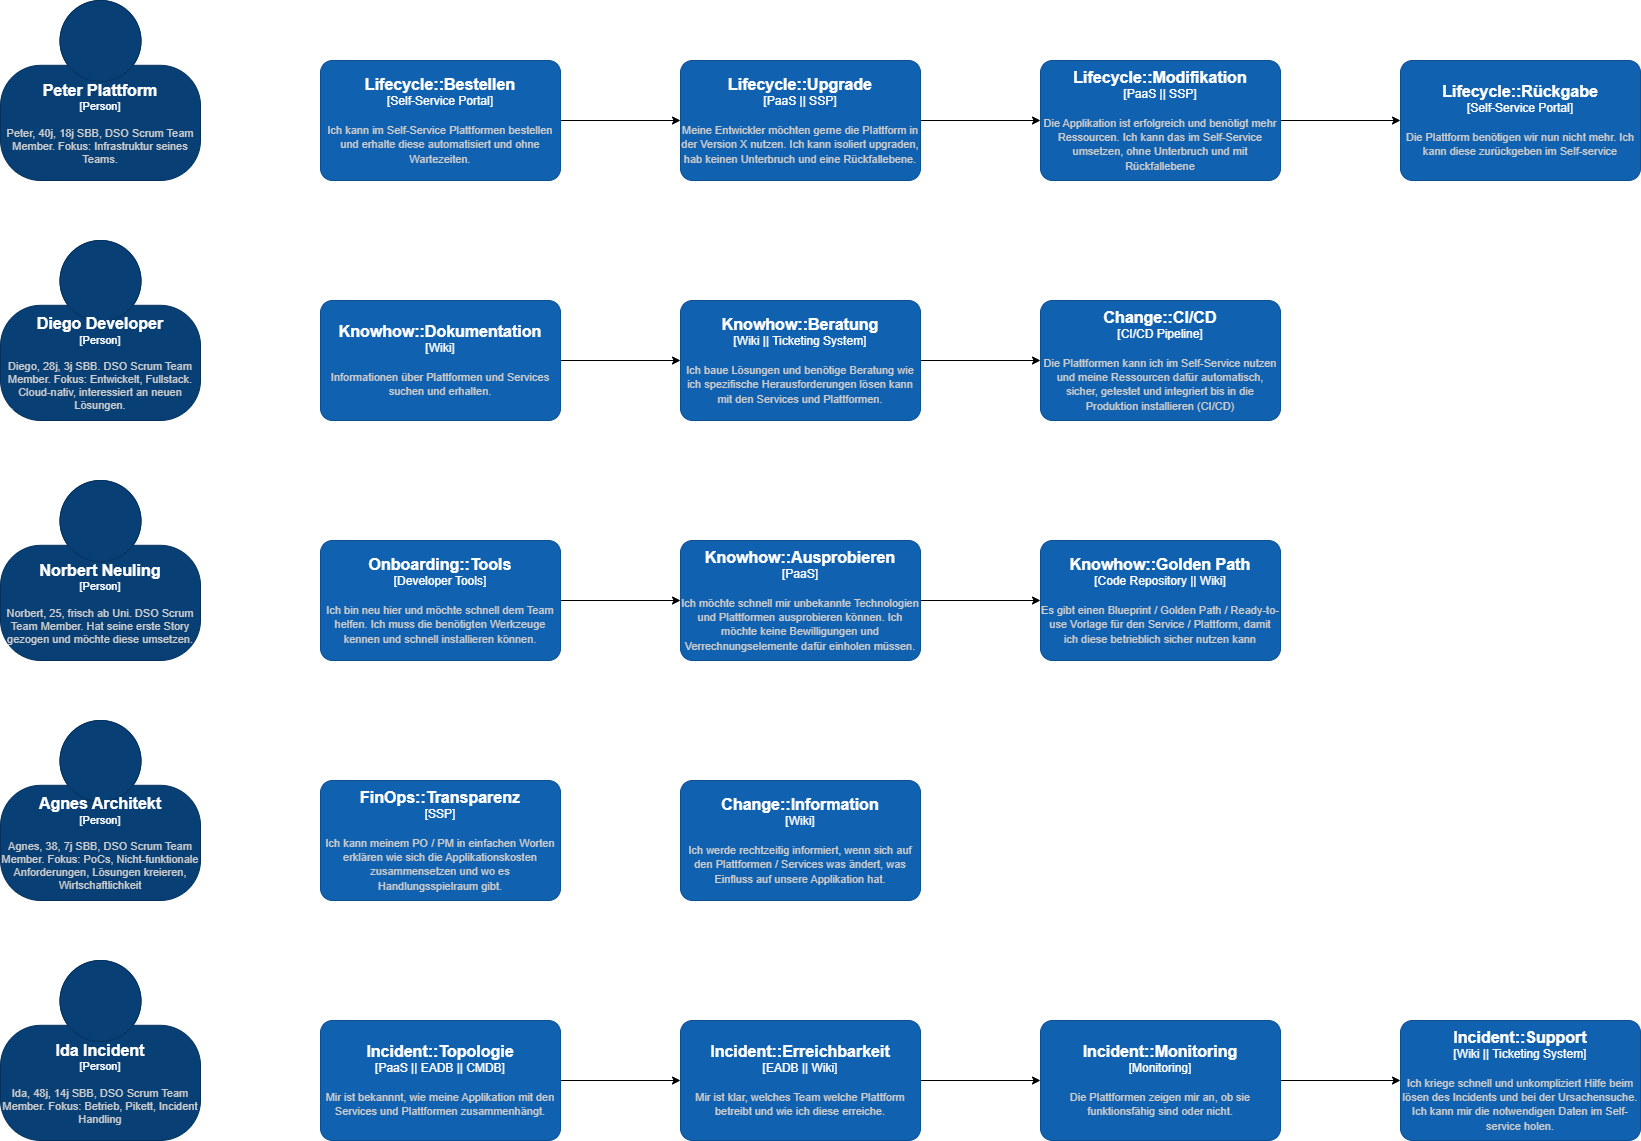
\includegraphics[angle=270,origin=c,width=\linewidth]{customer-journey.png}
        \caption{Customer Journey Map}
        \label{fig:customerjourney}
    \end{figure}

    \subsection{Survey}
    \label{subsec:survey}
    \begin{table}[!htbp]
        \begin{center}
            \begin{tabularx}{\textwidth}{lXll}
                \toprule
                Id & Question                                                                                                                                                                              & Mean & <3 \\
                \midrule
                1  & Auffindbarkeit von Informationen über die Plattformen und Services. Zb. Confluence, Ardoq, Intranet... & 0 & 0         \\
                2  & Ich kriege schnell und unkompliziert Beratung bei der Konzipierung von Applikationen, zb. für Engineering oder Development. & 0 & 0  \\
                3  & Qualität der Dokumentation der Plattformen und Services (Sowohl Umfang, Aktualität und Inhalt). & 0 & 0  \\
                4  & Onboarding, bis ich meine Werkzeuge für Dev oder Ops lokal installiert habe.                                                                                                          & 0 & 0  \\
                5  & Lifecycle von Infrastruktur im Selfservice, hier; ich kann Services und Plattformen schnell und unkompliziert ausprobieren.  & 0 & 0  \\
                6  & Lifecycle von Infrastruktur im Self-Service, hier Bestellen von Plattformen                                                                                                           & 0    & 0  \\
                7  & Lifecycle von Infrastruktur im Self-Service, hier, Upgrade von Plattformen / deiner Applikation auf den Plattformen & 0 & 0  \\
                8  & Lifecycle von Infrastruktur im Self-Service, hier Modifikation von Plattformen oder Applikationen. & 0 & 0  \\
                9  & Lifecycle von Infrastruktur im Self-Service, hier Run-Down oder Rückgabe von Plattformen & 0 & 0  \\
                10 & Es gibt einen Blueprint / Golden Path / Vorlage, die mir zeigt, wie ich eine Plattform verwenden kann. & 0 & 0  \\
                11 & Die Plattformen erlauben mir, meine Ressourcen automatisiert zu bauen und zu deployen (CI/CD) & 0 & 0  \\
                12 & Ich kann meinem PO die Kosten unserer genutzten Services und Plattformen nachvollziehbar erklären. & 0 & 0  \\
                13 & Ich verstehe, wie meine Applikation mit den Plattformen zusammenhängt bei Incidents & 0 & 0  \\
                14 & Welches DSRV Team für welche Plattform verantwortlich ist, ist mir klar.                                                                                                              & 0    & 0  \\
                15 & Ich kriege schnell und unkompliziert Hilfe im Incident Fall.                                                                                                                          & 0    & 0  \\
                16 & Die Plattformen zeigen mir an, ob sie funktionsfähig sind oder nicht. (zb. Monitoring, Chat, ...). & 0 & 0  \\
                17 & Ich, bzw. mein Team, werden rechtzeitig und mit genug Details informiert, wenn sich auf den Plattformen etwas ändert, was Auswirkungen auf die von uns verantwortete Applikation hat. & 0 & 0  \\
                \bottomrule
            \end{tabularx}
        \end{center}
    \end{table}


\end{document}